\section{Greedy Algorithms}

\emph{Formal definition}: the greedy algorithm "stays ahead" locally: meaning that is better than any other solutions, alternatively we can prove that a greedy algorithm's solution is optimal by transforming the know optimal solution for the problem, into our solution, this method is called "argument exchange".\\\\\emph{Practical definition}: A lot of the time a greedy algorithms involves scanning all the $n \in INPUT$ of the problem, if the current element respect some conditions, then it can be added to the optimal solution returned by the algorithm.

\subsection{The Cashier Problem / Coin changing}

Given a currency with the following values: 1, 5, 10, 25, 100, devise a method to pay amount to customer using fewest number of coins.\\\\
\emph{Example}: 34 dollars, how many coins?\\\\
\emph{Solution}: at each iteration, add coin of the largest value that does not take us past the amount to be paid.

\begin{algorithm}[H]
    \SetAlgoLined
    \small
    \KwIn{$amount$ containing the amount to give back to the client, $C$ set containing all the coins of the current currency. }
    \KwOut{$S$ the set containing all the coins to give back to the client}
    \BlankLine


    $S \leftarrow$ set containing all the coins to give back to the client\;
    $total = 0 \leftarrow$ total expressed in the current currency system\;
    $Cs \leftarrow$ set containing all the coins in the currency sorted by increasing values\;

    \BlankLine
    \While{$total < amount $}{
        \For{i=Cs.length to 0 }{
            \uIf{$total + Cs[i] < amount$}{
                $ total = total + Cs[i]$\;
                $S = S \cup Cs[i]$\;
                $break;$
            }
            \uElseIf{$total + Cs[i] = amount$}{
                $S = S \cup Cs[i]$\;
                $ return \; S$\;
            }{}
        }

    }
    \BlankLine

    return $S$\;
    \caption{cashierAlgorithm(amount,C):}
\end{algorithm}

\begin{claim}
    The cashier algorithm always returns an optimal solution.
\end{claim}
\begin{proof}
    The aim of the algorithm is to give as little change as possible (in terms of number of coins), if this is not true, then it must exist a solution $|S^{*}| < |S|$, but the algorithm always give highest compatible coin in the for loop, therefore a contradiction.
\end{proof}\

\subsection{Interval Scheduling}

We have a set J of jobs to execute on a machine and $\forall j \in J \; j=(s_{j},f_{j})$ where s and f are start and finish.Two jobs are compatible if the don't overlap: $\forall j_{i},j_{j} \in C \; f_{i} \geq s_{j} \; or \;vice-versa $.\\
Once we defined the problem, is just the matter of identifying the best strategy to sort all the jobs in J. Turns out, the best strategy is to sort all the jobs by finishing time, from first to last (for a former proof please check the professor's slide, but the main idea is to prioritize the jobs that release the machine as soon as possible).

\begin{algorithm}[H]
    \SetAlgoLined
    \small
    \KwIn{$J$ set containing all the jobs}
    \KwOut{$S$ the set containing all the compatible jobs}
    \BlankLine

    $S \leftarrow$ set containing all the compatible jobs\;
    $Js \leftarrow$ set containing all the sorted jobs in increasing order of finishing time $f1 < .... f_{j}$

    \BlankLine
    \For{i=0 to Js.lenght }{
        \If{$J[i].start \geq S.last.finish$}{
            $S = S \cup Js[i]$
        }
        {}
    }

    \BlankLine

    return $S$\;
    \caption{earliestFinishingTime(J):}
\end{algorithm}

\begin{claim}
    The earliestFinishingTime always return an optimal solution.
\end{claim}
\begin{proof}
    Assume this is not true, then it must exist a solution $|S^{*}| > |S|$,containing at least one more compatible job, but the algorithm check every job in J, therefore a contradiction.
\end{proof}\\

\begin{claim}
    The complexity of the algorithm is $\mathcal{O}{(nlogn)}$
\end{claim}
\begin{proof}
    The for loop costs $\mathcal{O}{(n)}$, while, as stated before, the sorting costs $\mathcal{O}{(nlogn)}$, since $\mathcal{O}{(nlogn)} > \mathcal{O}{(n)}$, the whole algorithm is $\mathcal{O}{(nlogn)}.$
\end{proof}\\

\subsection{Interval Partitioning}
Assuming we have a set of lectures L and, $\forall l \in L ,\; l=(s,f)$ where s and f are start time and finishing time, find the minimum amount of classroom tho schedule all the lectures, so that no two lectures overlap in the same classroom (the definition of overlap is the same as 3.2).

\begin{algorithm}[H]
    \SetAlgoLined
    \small
    \KwIn{$L$ set containing all the lectures}
    \KwOut{$S$ set containing the minimum amount of classroom needed}
    \BlankLine

    $S \leftarrow$ set containing the minimum amount of classroom needed\;
    $Ls \leftarrow$ set containing all the sorted lectures in increasing order of starting time $s1 < .... s_{j}$

    \BlankLine
    \For{i=0 to Ls.lenght }{
        $C = \varnothing$

        \uIf{$J[i].start \geq C.last.finish$}{
            $C = C \cup Ls[i]$\;
        }
        \Else{
            $S = S \cup C$\;
            $C = \varnothing$\;
            $C = C \cup Ls[i]$\;
        }
    }

    \BlankLine

    return $S$\;
    \caption{intervalPartitioning(L):}
\end{algorithm}

The number of classrooms needed is more or equal to the depth of $|S|$, that is also the maximum amount of items that contains at any given time.	\\

\begin{claim}
    The intervalPartitioning always return an optimal solution.
\end{claim}
\begin{proof}
    Same as 3.2, if it exist a better solution $S^{*}$ we would have $|S^{*}| > |S|$ but that is not possible, since the algorithm checks every lecture in the input set.
\end{proof}\\

\begin{claim}
    The complexity of the algorithm is $\mathcal{O}{(nlogn)}$
\end{claim}
\begin{proof}
    Identical as 3.2.
\end{proof}\\

\subsection{Minimizing The Lateness}
Assuming now we have just one resource that can process just one job at a time, we want to process all possible jobs. For the notation: $\forall j \in J,$ j requires  $t_{j}$ amount  of time to be executed, with a finishing time $f_{j} = s_{j} + t_{j}$, we have also to define a due date $d_{j}$ and finally the lateness of a job as: $max (0,d_{j}-f_{j})$

\begin{algorithm}[H]
    \SetAlgoLined
    \small
    \KwIn{$L$ set containing all the lectures}
    \KwOut{$S$ set containing the minimum amount of classroom needed}
    \BlankLine

    $S \leftarrow$ set containing all the compatible jobs\;
    $Js \leftarrow$ set of all jobs sorted by increasing deadline $s1 < .... d_{j}$

    \BlankLine
    $t = 0 $\;
    \For{i=0 to Js.lenght }{
        $s_{i} = t$\;
        $f_{i} = s_{i} + Js[i].finish$\;
        $S = S \cup (s_{i},f_{i})$\;
        $t = t + Js[i].time$\;
    }

    \BlankLine

    return $S$\;
    \caption{earliestDeadLineFirst(J):}
\end{algorithm}

\begin{claim}
    EarliestDeadLineFirst algorithm return an optimal solution.
\end{claim}
\begin{proof}
    Identical as 3.2 / 3.3.
\end{proof}\\

\begin{claim}
    The complexity of the algorithm is $\mathcal{O}{(nlogn)}$
\end{claim}
\begin{proof}
    Identical as 3.2.
\end{proof}\\

\clearpage

\subsection{Dikstra Algorithm}

\emph{Def}: A path is a sequence of edges which connects a sequence of nodes.\\\\
\emph{Def}: A cycle is a path with no repeated nodes or edges other than the
starting and ending nodes.\\\\
\emph{Shortest Path problem}: Given a digraph G = (V, E), edge lengths $le \geq 0$, source $s \in V$, and destination $t \in V$, find the shortest directed path from s to t.

\begin{figure}[H]
    \centering
    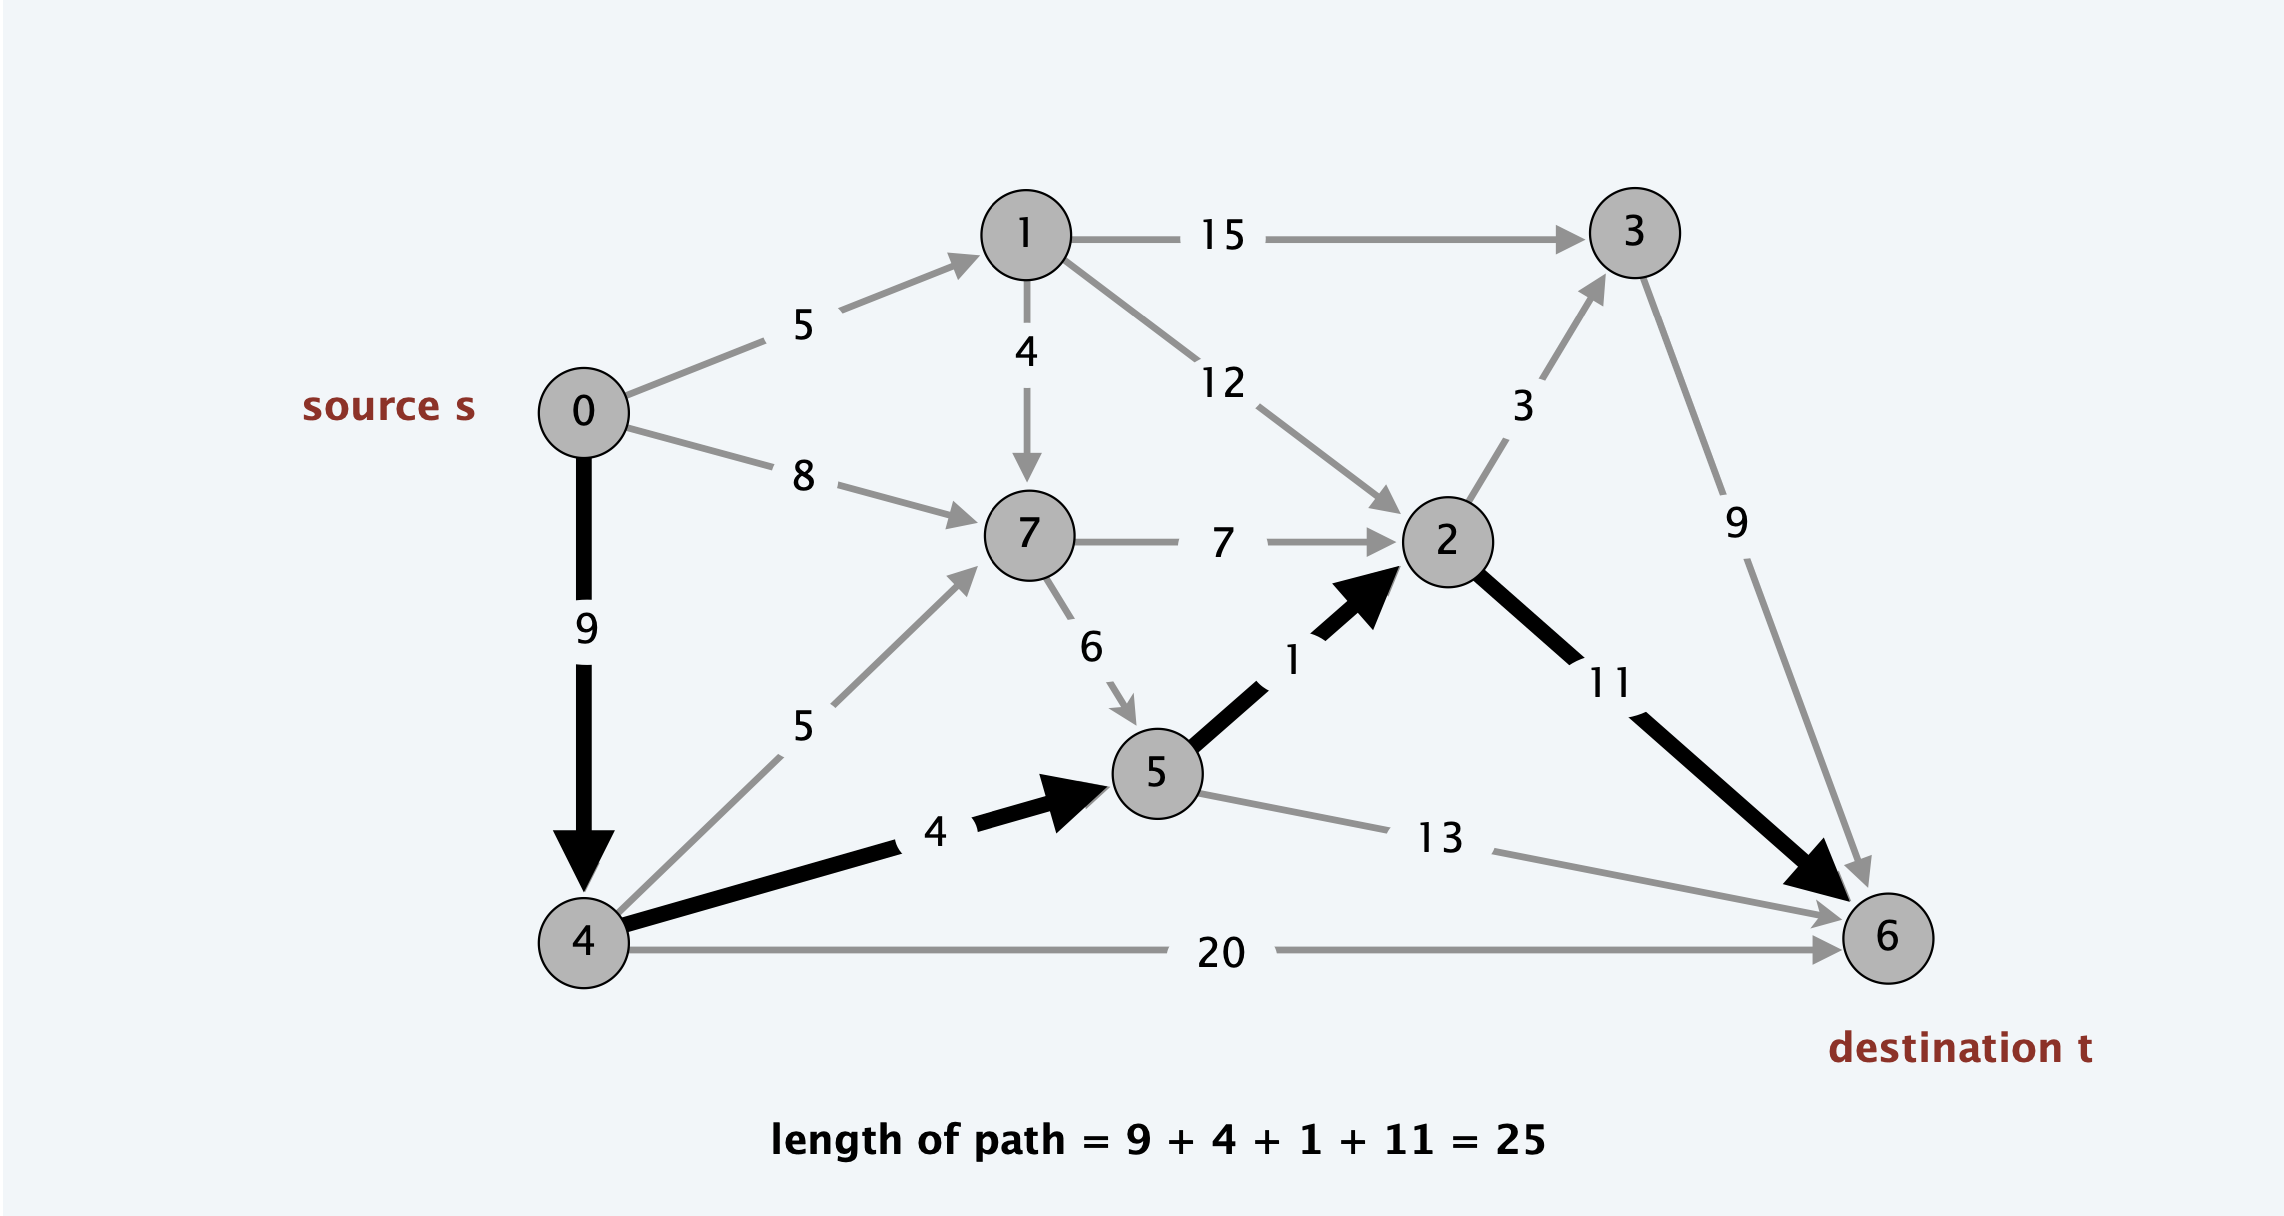
\includegraphics[width=0.8\textwidth ]{dikstra}
    \caption{A solution for the Shortest path problem.}
\end{figure}

\begin{algorithm}[H]
    \SetAlgoLined
    \small
    \KwIn{$G$ set containing all the edges of G, $s$ source of the path}
    \KwOut{$S$ set containing all the edges of a shortest path}
    \BlankLine

    $S \leftarrow$ set containing all the compatible jobs\;
    $Q \leftarrow$ priority queue for nodes contained in the unexplored part of G \;
    $D \leftarrow$ set of distances from s $\forall \; e \in G$

    \BlankLine

    $d(s,s) = 0$\;
    $D = D \cup d(s,s))$\;

    \BlankLine

    \For{i=0 to G.lenght }{
    $e_{i} = G[i] \leftarrow$ current edge to check\;
    \uIf{$e_{i} \neq s$}{
    $d(s,e_{i}) = \infty$\;
    $D = D \cup d(s,e_{i}))$\;
    $Q = Q \cup (e_{i},d(s,e_{i})) \leftarrow$ Insert in queue the current node with key($e_{i}$) = $d(s,e_{i})$\;
    }
    }

    \BlankLine

    \While{$Q \neq  \emptyset$}{
        $u = Q.getMin $\;
        $Q = Q - \{u\} $\;
        \ForEach {$(u,v) \in G, \; leaving \; u $}{
            \uIf{$d(s,v) > d(s,u) + l(u,v)$}{
                $S = S \cup  d(s,u) + l(u,v) $\;
                decrease-key of v to d(u) + l(u, v) in Q.\;
            }
        }
    }

    return $S$\;
    \caption{Dikstra(G,s):}
\end{algorithm}

\begin{claim}
    The Dikstra Algorithm always return an optimal solution ($\forall u \in S, \; d(u)$ is the length of the shortest $s\rightarrow u$ path).
\end{claim}
\begin{proof}
    Base case: $| S |$ = 1 is easy since S = { s } and d(s) = 0, assume that's true for $| S | > 1$:\\
    let t be next node added to S, and let (u, t) be the final edge: the shortest $s\rightarrow u$ path + (u, t) = $s\rightarrow t$ path of length $π(t)$.\\\\Now consider any $s\rightarrow t$ path P: it's is no shorter than $π(t)$. Let (x, y) be the first edge in P that leaves S, and let P' be the subpath to x, P is already too long as soon as it reaches y, so putting all together:
    \[l( P ) \geq l( P ' ) + l( x , y ) \geq d ( x ) + l( x , y ) \geq π ( y ) \geq π (t)\]
\end{proof}\\

\begin{claim}
    The Dikstra Algorithm complexity, for a graph G=(V,E), using a priority queue is: $\mathcal{O}{((V + E) \; log\; V)}$.
\end{claim}

\begin{proof}
    It highly depends on the type of queue used, but we have to check all the nodes in the priority queue plus all the edges coming out of every node, for further detail, please check the professor's slides.
\end{proof}\\


\subsection{Kruskal Algorithm}
Given an undirected, weighted, connected graph G=(V,E) we want to find the all the edges that connects all the nodes with a minimum cost, alternatively we can say that the algorithm finds the minimum spanning tree (MST) of G.\\\\
\emph{Formal definition}: Given an undirected, weighted, connected  graph G = (V, E) with edge costs $c(e)$, an MST is a subset of the edges $T \subseteq E$ such that T is a spanning tree whose sum of edge costs is minimized.

\begin{figure}[H]
    \centering
    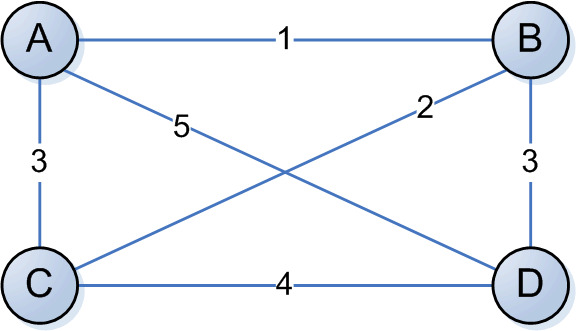
\includegraphics[width=0.4\textwidth ]{kruskal}
    \caption{An instance of the MST problem.}
\end{figure}

\begin{figure}[H]
    \centering
    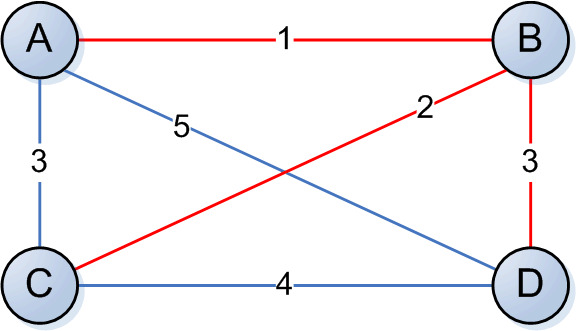
\includegraphics[width=0.4\textwidth ]{kruskal_solved}
    \caption{A solution for the MST problem.}
\end{figure}

\begin{algorithm}[H]
    \SetAlgoLined
    \small
    \KwIn{$G$ set containing all the edges of G}
    \KwOut{$S$ set containing all the edges of MST}
    \BlankLine

    $S \leftarrow$ set containing all the compatible jobs\;
    $E \leftarrow$ set of all the edges sorted by increasing weight $c(e)_{1} < .... c(e)_{j}$

    \BlankLine

    \For{i=0 to G.lenght }{
        $e_{i} = G[i] \leftarrow$ current edge to check\;
        \uIf{$S \cup e_{i} \;is \;not \;a \;loop$}{
            $S = S \cup e_{i}$ \;
        }
    }

    \BlankLine

    return $S$\;
    \caption{kruskal(G):}
\end{algorithm}

\begin{claim}
    Kruskal algorithm returns an optimal solution.
\end{claim}
\begin{proof}
    Identical as 3.2 / 3.3.
\end{proof}\\

\begin{claim}
    The complexity of the algorithm is $\mathcal{O}{(nlogn)}$
\end{claim}
\begin{proof}
    Identical as 3.2.
\end{proof}\\

\clearpage
